% Asset ID: A21NumericalMethodsTikZ-007
% Source: CCEA specification map + Chapter 10 Numerical Methods evidence
% Related section: A21 Numerical Methods lesson
% Purpose: Staircase and cobweb.
\documentclass[tikz,border=8pt]{standalone}
\usetikzlibrary{arrows.meta,positioning}
\begin{document}
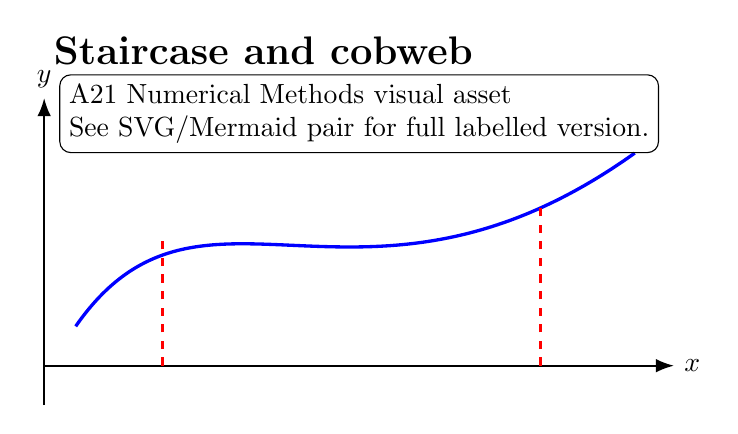
\begin{tikzpicture}[>=Latex]
\node[anchor=west,font=\Large\bfseries] at (0,4) {Staircase and cobweb};
\draw[->,thick] (0,0) -- (8,0) node[right] {$x$};
\draw[->,thick] (0,-0.5) -- (0,3.4) node[above] {$y$};
\draw[very thick,blue] (0.4,0.5) .. controls (2,2.8) and (4,0.2) .. (7.5,2.7);
\draw[very thick,red,dashed] (1.5,0) -- (1.5,1.6);
\draw[very thick,red,dashed] (6.3,0) -- (6.3,2.1);
\node[draw,rounded corners,align=left] at (4,3.2) {A21 Numerical Methods visual asset\\See SVG/Mermaid pair for full labelled version.};
\end{tikzpicture}
\end{document}
